\chapter{Week 12}

    \section{JupyROS Presentation}

    This week I prepared a JupyROS demonstration and presented it to the lecturers of the Automated and Connected Driving Challenges (ACDC) at RWTH. The team expressed interest in using JupyROS and incorporating it into their course material.

    Having gone through all the functions in the \texttt{jupyter-ros} and \texttt{jupyterlab-ros} packages, it was noticed that a few small modifications could be made to improve the user experience.

    For the JupyterLab extension:
    \begin{itemize}
        \item specify what the \textit{default} ROS path is in the settings,
        \item have an indication when new paths are saved,
        \item and make the ROS bag widget compatible with the dark theme.
    \end{itemize}

    And for \texttt{jupyros}:
    \begin{itemize}
        \item include the \texttt{ipycanvas} dependency so that the \texttt{turtlesim} widgets work out of the box,
        \item and make the axis labels for the live-plotting widget configurable or default to \textit{time} on the $x-$axis since this will be the most common use case.
    \end{itemize}

    \section{URDF Extension III}

    Continuing with the URDF extension, the challenge for this week was to load the contents of a URDF file and be able to add the 3D objects to the scene in the widget. The initial attempt involved following Garrett Johnson's example to create a simple scene and add a six-legged robot to it. 

    \begin{lstlisting}[language=typescript]
scene = new Scene();
scene.background = new Color(0x263238);

renderer = new WebGLRenderer({ antialias: true });
this.node.appendChild(renderer.domElement);

const directionalLight = new DirectionalLight(0xffffff, 1.0);
scene.add(directionalLight);

const ambientLight = new AmbientLight(0xffffff, 0.2);
scene.add(ambientLight);

const ground = new Mesh(new PlaneBufferGeometry(), 
                        new ShadowMaterial({ opacity: 0.25 }));
scene.add(ground);
    \end{lstlisting}

    \noindent The creation of the scene was straight forward, however, the issues began when trying to load the robot's mesh files. The extension on it's own is unable to find local files unless there is a server providing those files. 
    
    \begin{lstlisting}[language=typescript]
// Load robot
const manager = new LoadingManager();
const loader = new URDFLoader(manager);
loader.load('../../../urdf/T12/urdf/T12_flipped.URDF', result => {
    robot = result;
});
    \end{lstlisting}

    \noindent The workaround for this was to use \href{https://github.com/RoboStack/amphion}{Amphion} which uses \href{https://github.com/rapyuta-robotics/urdf-js}{\texttt{urdf-js}}, a derivative of the \texttt{urdf-loaders} package. Amphion works with ROS to find the mesh files indicated in a URDF file. As long as the mesh files are included in a ROS package such as \texttt{panda\_description}, the extension will be able to locate and load the files by using Amphion. 

    Several issues were encountered when attempting to use Amphion itself with the extension, but once the developers had corrected the configuration of the extension, robots could finally be visualized in the widget as seen in Figure \ref{fig:urdfSpot}. For this example, all the mesh files had to be converted to \texttt{.stl} from the original \texttt{.obj} extension; and a ROS package called \texttt{spot\_description} was created to include all the mesh files. Once the environment was sourced properly, the URDF extension was able to locate all the necessary files.

    \begin{figure}[H]
        \centering
        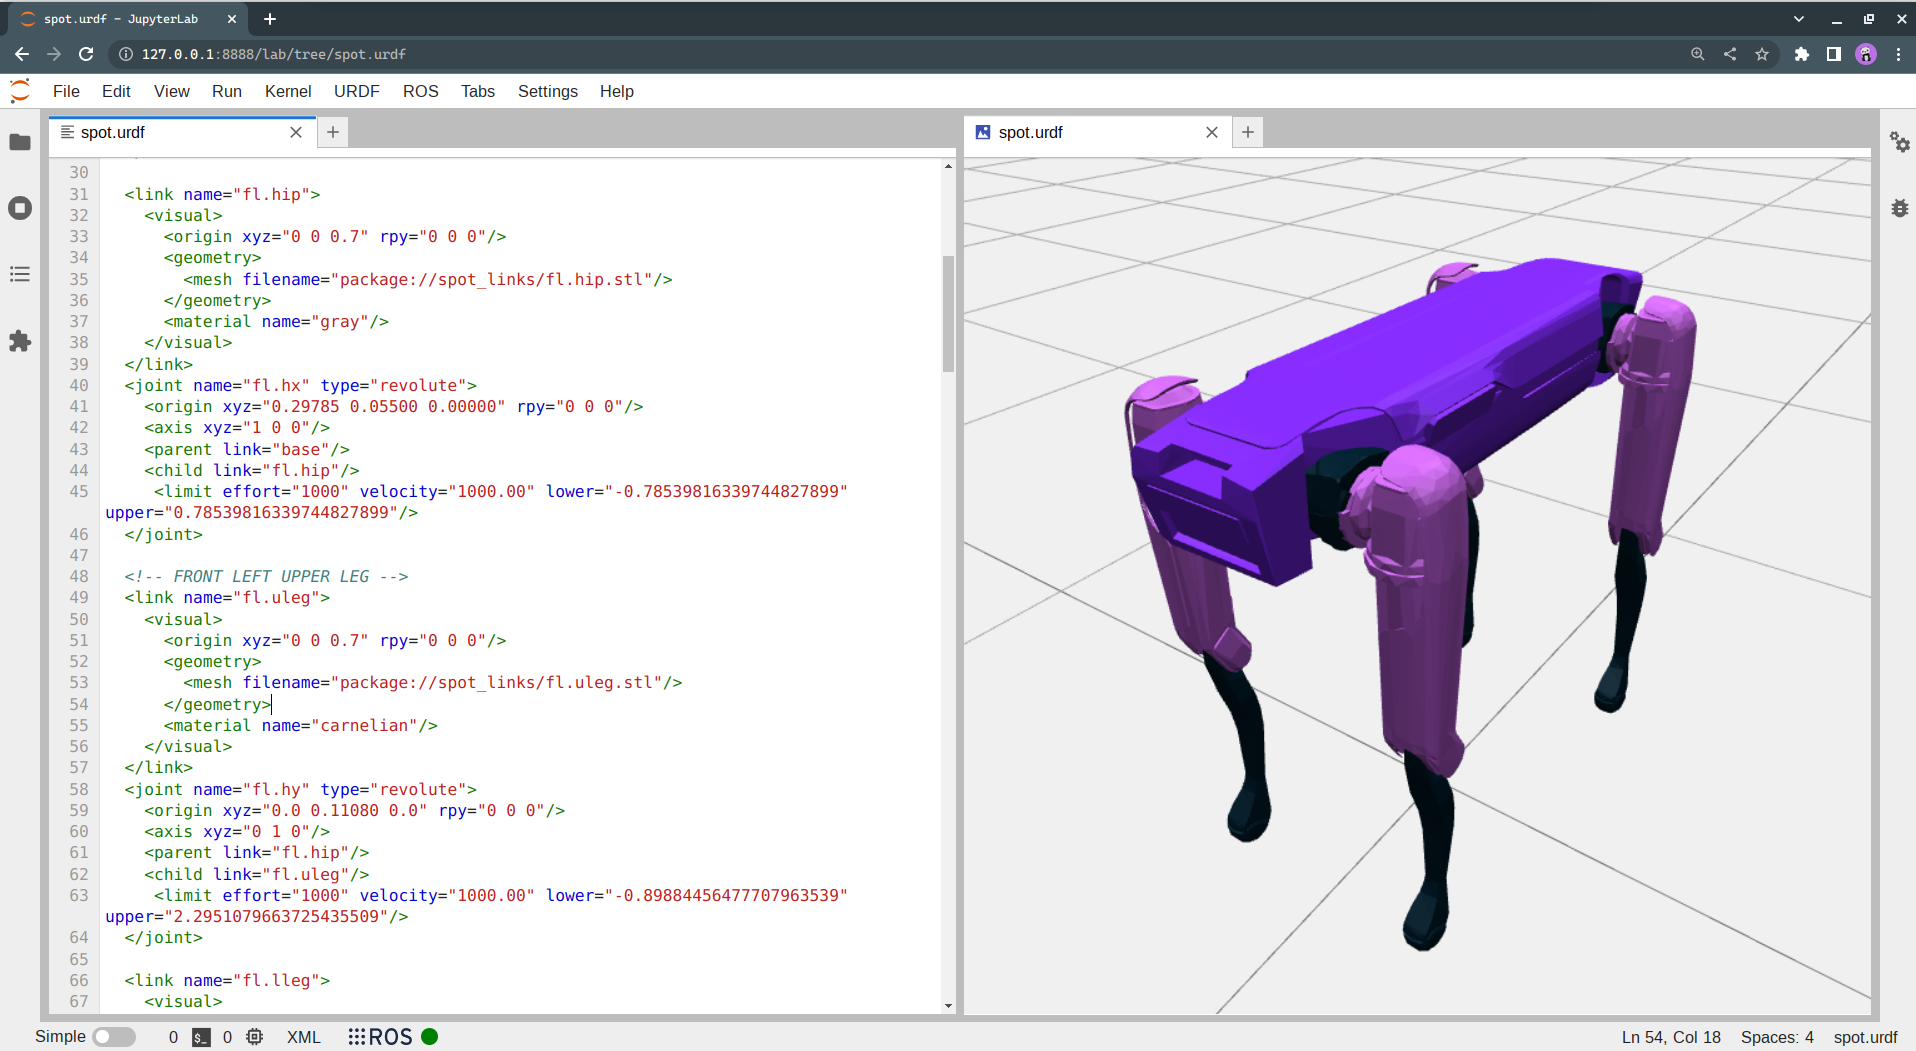
\includegraphics[width=\linewidth]{Images/12_urdfSpot.png}
        \caption{The resulting robot display after the incorporation of Amphion for loading ROS package files}
        \label{fig:urdfSpot}
    \end{figure}

    \section{Future Work}
    
    The next steps will be to finalize the URDF extension, this will include giving the user more options for configuring the scene such as changing the background and moving the robot joints manually. Additionally, documentation needs to be written for the extension so that users can easily set up and work through any of the given examples.
